%\section{Design of MuLeS}
\section{MuLeS's Design and Implementation}
\label{sec:proposal}

In the following, Section \ref{subsec:networkmodel} describes the network model. We then formulate our targeted problem in Section \ref{subsec:proposeddesign}, and provide our implementation in Section \ref{subsec:implement}.


\subsection{Network model}
\label{subsec:networkmodel}

\begin{figure}[t]
\centering
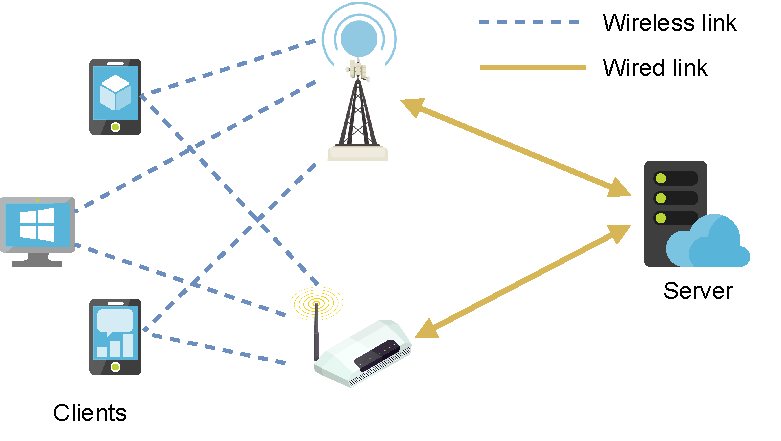
\includegraphics[width=9cm]{figs/ccnc-networkmodel2.pdf}
\caption{\textbf{The multi-client network model.} A server simultaneously transmits data to clients equipped with multiple network interfaces.} \label{fig:networkmodel}
%\vspace{-0.6cm}
\end{figure}

% Le &Trung's text
%\figureref{fig:networkmodel} depicts our network model, where MPQUIC mobile clients connect to an MPQUIC server through two network interfaces (e.g., Wi-Fi and LTE/5G), each forms a path with certain level of dynamicity. 
%Kien's text 2023 Sep. 3
\figureref{fig:networkmodel} depicts our network model, where several MPQUIC clients connect to an MPQUIC server. A client has two network interfaces (e.g., Wi-Fi and LTE/5G), each forming a path with a certain level of dynamicity. We consider a download scenario at the server in which the scheduler determines the optimal path for transmitting each subsequent packet upon receiving a download request. A successfully connected client $j$ is managed by the server by a session, denoted as \textbf{session $c_j$}. In this session, a path is characterized by the following parameters: 
\begin{itemize}
    \item \textbf{sRTT}: stands for Smooth Round Trip Time, which is defined by $\frac{1}{8}$lRTT + $\frac{7}{8}$sRTT \cite{rfc9002}, where lRTT depicts the latest Round Trip Time up to the current time step $t$.
    \item \textbf{RTT variation}: refers to the fluctuation or inconsistency of RTT over time. %In the context of path scheduling algorithms in MPQUIC, RTT variation serves as a fundamental parameter.
    \item \textbf{Packet loss}: represents the ratio of the number of lost packets, including retransmission packets, to the total number of packets sent during data transmission. A sent packet is marked as lost if the sender has not received the acknowledgment packet (ACK) within a specified period.   
    %The time threshold is $k_{TimeThreshold} * max(sRTT, lRTT)$. The loss rate refers to the ratio of the number of lost packets, including retransmission packets, to the total number of packets sent during data transmission.
    \item \textbf{Congestion window (CWND)}: determines the amount of data that can be sent before receiving an ACK. 
\end{itemize}
% Kieh changed the heading
\subsection{Multi-client Learning-based MPQUIC scheduler}
\label{subsec:proposeddesign}
In the following, we first define agents, states, and actions. We then propose the reward function and path selection policy.
\noindent \textbf{Agent:}
In the reinforcement learning paradigm, an agent is an entity that interacts with the environment to learn and execute actions to achieve the goal. In the packet scheduling context, we consider the server an agent and offer a scheduling strategy to minimize the average download time of all packets. 

\noindent \textbf{States and actions:} A state should contain all the information that supports the agent in deciding the action. However, incorporating excessive information in the state may result in a large Q-table, leading to extra training time. Therefore, it is crucial to include only essential information. In MPQUIC scheduling, the agent's ultimate goal is to determine appropriate paths to transmit the upcoming packets. We observe that CWND and RTT are the most valuable indicators of a path's accessibility. Therefore, we suggest a state comprising information related to CWND and RTT. 

Suppose at the time step \textit{t}, there are \textit{m} packets $\{p_1, \ldots p_m\}$ to transmit. Without loss of generality, we suppose that these \textit{m} packets belong to sessions $\{c_1, c_2, \dots, c_m\}$, respectively.
%Hai 
For each session $c_j$, we define its corresponding state as a tuple $S^t_{j} = \{s^t_{j}, \overbar{s^t_{j}}\}$, where $s^t_{j}$ represents state of current session $c_j$ and $\overbar{s^t_{j}}$ is the state of remaining sessions. 
%Hai
$s^t_{j}$ and $\overbar{s^t_{j}}$ are $n$ dimensional vectors, whose $i$-th element presents information related to the $i$-th path.  
Specifically, the $i$-th element of $s^t_{j}$ (resp. $\overbar{s^t_{j}}$), denoted as $s^t_{i,j}$ (resp. $\overbar{s^t_{i,j}}$), is defined as follows:
\begin{eqnarray}
\label{eq:state_r}
%\begin{split}
    s^t_{i,j} &= &\frac{\frac{CWND_{i,j}}{{lRTT_{i,j}}}}{\sum_{k=1}^{n} \frac{CWND_{k,j}}{{lRTT_{k,j}}}}, \\
    \overbar{s^t_{i,j}} &= & \frac{1}{m-1}\left (\sum_{j=1}^{m} \frac{\frac{CWND_{i,j}}{{lRTT_{i,j}}}}{\sum_{k=1}^{n} \frac{CWND_{k,j}}{{lRTT_{k,j}}}} - s^t_{i,j} \right ),
%\end{split}
\end{eqnarray}
where $CWND_{i,j}$ and $lRTT_{i,j}$ depict CWND size and latest RTT up to the current time of path $i$-th at session $c_j$, respectively. Since $s^t_{i,j}$ is a continuous value in the range [0,1], we discretize the value of $s^t_{i,j}$ into five values, including [0,0.3), [0.3,0.4), [0.4,0.5), [0.5,0.6), and [0.6,1] to create state-action pairs. For each packet $p_j$, the agent takes its state vector $S^{t}_j$ and uses the scheduling policy (described later) to decide the action, which is choosing the path for transmission.

% Trung & Le's text
%\noindent \textbf{Reward function:} The reward function plays a crucial role in guiding the agent's actions. In the case of the MPQUIC scheduling, the ultimate goal is to minimize all flows' download time. Consequently, the selected paths should prioritize minimizing the RTT and reducing the loss rate. With this in mind, we design a simple yet effective reward function that incorporates two key factors as below:

% Kien's text
\noindent \textbf{Reward function:} The reward function is crucial in guiding the agent's actions. In MPQUIC scheduling, the ultimate goal is to minimize all flows' download time. Consequently, the selected paths should prioritize shortening RTT and reducing the loss rate. With this in mind, we design a simple yet effective reward function that incorporates two key factors:
\begin{align}
\label{eq:reward}
\begin{split}
R{(S^t_{j}, a^t)}=
\begin{cases}
   - lRTT_{j} & \text{, if received ACK} \\
  - \beta & \text{, if packet loss},
  % & n>1
\end{cases}
\end{split}
\end{align}
where $lRTT_{j}$ is the value of the latest RTT at session $c_j$, and $\beta > 0$ is a tunable parameter. 
We prioritize actions that minimize the packet transmission delay by penalizing $lRTT_{t,j}$. Moreover, by introducing the term $-\beta$, we encourage the agent to alleviate packet loss.

\noindent \textbf{Q-table and policy:} 
The Q-table stores the estimated values of actions with respect to different states. Specifically, $q(i,j)$ demonstrates the goodness of performing action $a_i$ at state $S_j$. We leverage the $\epsilon$-greedy-based policy to decide the action (see Algorithm \ref{algo:qlearning}). At each time step $t$, for each packet $p_j$, we choose the path with the highest Q-value with a probability of $1-\epsilon$ and choose a path with minimal RTT with a probability of $\epsilon$. After taking action, the agent uses the equation (\ref{eq:bellman}) to update Q-learning's elements related to state $S_{j}^t$.
% Initially, we initialize all elements of the Q-table with zeros. 
% \textcolor{blue}{At each time step $t$, after taking action, the agent uses the Bellman Equation (~\ref{eq:bellman}) to update Q-learning's elements related to state $S_{j}^t$.
% }
% In the learning stage, MuLeS updates the values of state $S_{j}^t$ in the Q-table according to Equation~\ref{eq:bellman}. Where $S_{j}^t$ is determined by the Equation~\ref{eq:state_r}, consisting of pairs of vectors $\{s_j^t, \overbar{s_j^t}\}$ reflecting the state at session $c_j$ (which receives the reward) and at the remaining available sessions in the network, respectively.

% \noindent \textbf{Policy-based scheduling decision}: MuLeS selects a path based on the action value, that is, the path with a higher Q value, as presented in Algorithm \ref{algo:qlearning}. In addition, MuLeS defines an epsilon value ($\varepsilon$) to balance between exploiting current knowledge (choosing actions with the highest Q-values) and exploring new actions (based on minRTT logic) to discover better strategies.

%\noindent \textbf{Path selection policy:}
%The server selects a path based on the action value, that is, the path with a higher Q value is chosen as the \textit{prioritized path}, as is presented in Algorithm \ref{algo:qlearning}. If the \textit{ priority path} is available (that is $\frac{BiF}{CWND} < 1$), it is chosen to transmit the upcoming packet. Otherwise, if the remaining path is available and has an sRTT lower than that of the \textit{prioritized path}, then the remaining path is chosen instead. If all of these conditions are not satisfied, the server waits until the next time step. 
\begin{algorithm}
\caption{MuLeS's scheduling for $j$}\label{algo:qlearning}
 % Sessions $\mathcal{SS} = \{ss_1, ss_2, \dots, ss_m\}$\\
 Paths $\mathcal{P} = \{a_1, a_2, \dots, a_n\}$\\
 States $\mathcal{S} = \{S_j^t = \{s_j^t, \overbar{s_j^t}\}\}$\\ 
 Actions $\mathcal{A} = \mathcal{P}$\\
 Q-table $Q: \mathcal{S} \times \mathcal{A} \rightarrow \mathbb{R}$\\
 Epsilon $\varepsilon \in [0, 1]$\\
\small
\SetAlgoLined
% \Input{number of state;}
\Begin{$t \gets 0$, Let $Q(s,a)=0 ~ \forall (s,a) \in \mathcal{S} \times \mathcal{A}$\\
    % \emph{// calculate the priority of each experience $(S_{t,j}, S_{t+1,j}, a_t)$};\\
    \For{$t$}{
        \eIf{$random(0,1) > \varepsilon$}{
            Observe state $S_{j}^t \in \mathcal{S}$\\
            $p_t \gets argmax(Q \mid S=S_{j}^t)$
        }{
        $p_t \gets$  minRTT scheduler;
        }
    }
}

\end{algorithm}

\subsection{Implementation}
\label{subsec:implement}
We implement MuLeS as an MPQUIC scheduler using the Golang code base introduced in~\cite{mpquic}. MuLeS includes three primary modules: MuLeS Controller, Path selector, and Handler, as shown in \figref{fig:fqsatimplement}.\\
\noindent \textbf{MuLeS Controller:} stores a \textit{Q-table} and serves as a central module outside structures that manage sessions. Hence, the controller can gather all sessions' information and make a scheduling decision for all clients. Whenever the server has a packet for transmission, it collects states of the corresponding sessions, utilizes the algorithm described in Section \ref{subsec:proposeddesign}, then chooses a path that is supposed to maximize reward. Notably, after sending the packet, the agent can not observe the reward immediately and must wait for an ACK instead. At that moment, the network state will be very different; thereby, it's essential to build a \textit{map that stores state information} for reward calculating and Q-table updating in the future. \\
\noindent \textbf{Path selector} and \textbf{Handler:} are two modules incorporated in each session. Path selector receives the Q-values from the controller and selects the appropriate path using the policy described in Section~\ref{subsec:proposeddesign}.
At the same time, Handler is responsible for calculating the reward value whenever receiving an ACK or detecting a packet loss.

% The former receives the 
% decision from the Controller and assigns the selected path to the flow.
% In the the state of the network at that session and making policy-based scheduling decisions as described in Section~\ref{subsec:proposeddesign}. At the same time, the \textbf{Handler} module is used to calculate the value of the reward function, whenever receiving an ACK or a packet lost.

\begin{figure}[t]
    \centering
    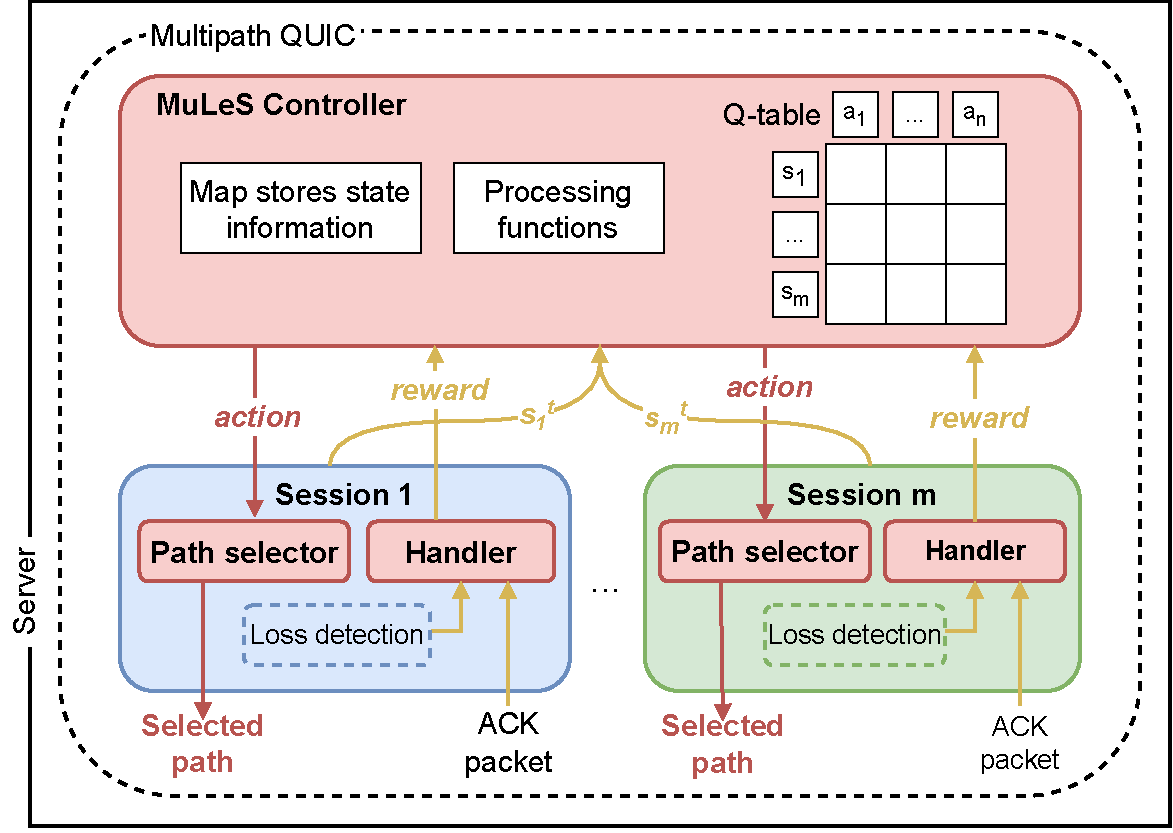
\includegraphics[width=8.8cm]{figs/ccnc-newdesign.pdf}
    \caption{MuLeS implementation in quic-go framework.}
    \label{fig:fqsatimplement}
\end{figure}

